\documentclass[12pt]{article}                                % [UNCHANGED]

%-----------------------------------------------------------------
%                          PACKAGES
%-----------------------------------------------------------------
\usepackage[margin=1in]{geometry}      % [UNCHANGED]
\usepackage{amsmath,amssymb,amsfonts}  % [UNCHANGED]
\usepackage{graphicx}                  % [UNCHANGED]
\usepackage{float}                     % [UNCHANGED]
\usepackage{booktabs}                  % [UNCHANGED]
\usepackage{caption}                   % [UNCHANGED]
\usepackage{subcaption}                % [UNCHANGED]
\usepackage{color}                     % [UNCHANGED]

\definecolor{darkgreen}{rgb}{0,0.5,0}

\usepackage{url}                       % [UNCHANGED]
\usepackage{xurl} % Allows URLs to break automatically
\usepackage[colorlinks=true, linkcolor=darkgreen, urlcolor=darkgreen, citecolor=darkgreen]{hyperref}
\usepackage{setspace}                  % [UNCHANGED]
\usepackage{amsmath}                   % [UNCHANGED]
\usepackage{algorithm}                 % [UNCHANGED]
\usepackage{algpseudocode}             % [UNCHANGED]
\usepackage{siunitx} % make sure siunitx is loaded

\DeclareSIUnit\ug{\micro\gram}
\DeclareSIUnit\m{\metre}

%-----------------------------------------------------------------
%                         BIBLIOGRAPHY
%-----------------------------------------------------------------
\bibliographystyle{plain}              % [UNCHANGED]

\begin{document}                       % [UNCHANGED]

%-----------------------------------------------------------------
%                          TITLE PAGE
%-----------------------------------------------------------------
\title{\textbf{Wildfire Smoke PM\textsubscript{2.5} Modeling with Convex Optimization and Low-Cost Sensors}\\   % [MODIFIED: Removed any leftover markdown styling]
       \large A Graph-Signal Approach to Data Recovery and Interpolation}                                   % [UNCHANGED]

\author{Param Somane \\                                   % [UNCHANGED]
        \small{University of California, San Diego} \\    % [UNCHANGED]
        \small{\texttt{psomane@ucsd.edu}}}                % [UNCHANGED]

\date{\today}                                             % [UNCHANGED]
\maketitle                                                % [UNCHANGED]

\begin{abstract}                                          % [UNCHANGED]
This report presents a comprehensive study on reconstructing and denoising wildfire smoke 
PM\textsubscript{2.5} sensor data using convex optimization and graph-based methods. By 
modeling sensors as nodes in a spatially informed graph, we apply Laplacian and total variation (TV) 
regularization to better handle missing or noisy readings. We compare these convex techniques 
(solved via ADMM, gradient descent) to classical spatial interpolation methods such as Kriging 
and IDW, with extensive cross-validation analyses under real-world low-cost sensor deployments. 
Our findings suggest that the proposed approach significantly improves interpolation accuracy 
while enhancing robustness to sparse connectivity and sensor outages.
\end{abstract}

\tableofcontents                                         % [UNCHANGED]

%-----------------------------------------------------------------
%                       I. INTRODUCTION
%-----------------------------------------------------------------
\section{Introduction}
\label{sec:intro}                                        % [UNCHANGED]

Wildfires emit large amounts of particulate matter, particularly PM\textsubscript{2.5}, causing 
severe air quality deterioration over extensive regions. 
\textbf{PM\textsubscript{2.5}} (particulate matter smaller than 2.5 micrometers in diameter) 
is especially concerning because such fine particles can penetrate deeply into the respiratory 
tract, leading to adverse health outcomes including respiratory and cardiovascular issues. 
Traditional regulatory monitoring networks (e.g., the U.S. EPA Air Quality System) are often 
too sparse to capture sharp local gradients and dynamic changes in smoke plumes, motivating 
the use of dense, low-cost sensor networks (e.g., PurpleAir).                                     % [MODIFIED: Removed leftover markdown styling, rephrased slightly]

Although these sensors provide high-resolution coverage, they pose challenges: noisy readings, 
biases at high concentrations, and frequent data gaps under extreme smoke~\cite{Barkjohn2022, 
PurpleAirUseCases}. To address these shortcomings, we explore a \textit{convex optimization} 
framework that exploits the spatial structure of sensor networks (encoded as a graph) to 
improve data accuracy and coverage.                                                               % [MODIFIED: unify wording, removed double asterisks]

\paragraph{Motivation and Previous Works.} % [UNCHANGED]
Recent years have seen multiple sensor-correction approaches~\cite{Barkjohn2022Sensors}, 
geostatistical methods (e.g., Kriging~\cite{ChilesDelfiner}), and data-fusion 
efforts~\cite{rapidfireGithub,rapidfireSupportCode} to refine PM\textsubscript{2.5} estimates. 
However, many do not adopt an explicit \emph{convex} formulation of the problem. Instead, 
they rely on statistical modeling or purely local correction factors. By contrast, we 
formulate a global optimization problem that can incorporate smoothness priors 
(via Laplacian or TV) while still honoring observed data.

\paragraph{Intended Contributions.}  % [UNCHANGED]
\begin{itemize}
    \item Propose a \textbf{graph-based convex optimization} approach (penalizing large 
    neighboring discrepancies) to fill missing sensor data and reduce noise.
    \item Compare new methods (ADMM, proximal gradient, Laplacian interpolation) against 
    \textbf{classical} baselines (IDW, Kriging).
    \item Provide a real-world case study using multiple CSVs of wildfire smoke sensor 
    data from Barkjohn \emph{et al.}, detailing how we integrate them and the 
    rationale behind each computational step.
\end{itemize}

\paragraph{Organization of the Paper.} % [MODIFIED: Slight rephrasing, but mostly unchanged content]
Section~\ref{sec:background} reviews relevant literature and fundamentals. 
Section~\ref{sec:problem-statement} gives the formal problem statement, primal-dual forms, 
and KKT conditions. Section~\ref{sec:data} details the dataset content and our preprocessing 
approach, while Section~\ref{sec:methods} describes our solver implementations (ADMM, 
gradient-based) and their relevance to our hypotheses. Section~\ref{sec:experiments} presents 
results of cross-validation and solver comparisons, followed by a broader discussion 
(Section~\ref{sec:discussion}) and conclusions in Section~\ref{sec:conclusion}.

%-----------------------------------------------------------------
%            II. BACKGROUND AND RELATED WORK
%-----------------------------------------------------------------
\section{Background and Related Work}
\label{sec:background}        % [UNCHANGED]

\subsection{Low-Cost Sensors in Wildfire Smoke Monitoring}    % [UNCHANGED]
Low-cost particle sensors (e.g., PurpleAir) have gained popularity for real-time monitoring of 
wildfire smoke events due to their affordability and dense spatial coverage~\cite{Barkjohn2022}. 
However, they can exhibit sensor-to-sensor variability, potential bias at high concentrations, 
and data gaps due to network or device issues. These drawbacks underscore the need for robust 
correction and data recovery methods.

\subsection{Convex Optimization in Environmental Data Recovery}   % [UNCHANGED]
Convex optimization provides robust frameworks for interpolating and smoothing environmental 
data, guaranteeing global optima under well-defined constraints/regularizers~\cite{BoydADMM}. 
Graph-based formulations often incorporate a Laplacian matrix to enforce smoothness across 
connected nodes (sensors). One may consider:
\begin{equation}
    \label{eq:laplacian-smoothing}
    \min_{\mathbf{x}} \;\; \frac{1}{2}\sum_{i \in \Omega} (x_i - y_i)^2 
    \;+\; \frac{\lambda}{2}\,\mathbf{x}^\top L \mathbf{x},
\end{equation}
where $\Omega$ is the set of sensors with valid data $y_i$, and $L$ is the graph Laplacian 
encoding adjacency. Such quadratic objectives are straightforward to solve, and the global 
optimum is guaranteed.

\subsection{Total Variation Minimization and Graph TV}   % [UNCHANGED]
Total variation (TV) regularization encourages piecewise-smooth solutions, allowing sharper 
transitions critical for delineating smoke plume boundaries~\cite{RudinOsherFatemi}:
\begin{equation}
    \label{eq:tv-smoothing}
    \min_{\mathbf{x}} \;\; \frac12\sum_{i \in \Omega} (x_i - y_i)^2 
    \;+\;\lambda \sum_{(i,j)\in E} |x_i - x_j|.
\end{equation}
TV is known to preserve edges in images or scalar fields—especially relevant for extreme 
wildfire “hotspots.”

\subsection{Baselines: Kriging and IDW}  % [UNCHANGED]
Classical geostatistical methods like \textit{Ordinary Kriging}~\cite{ChilesDelfiner} model 
spatial correlation via a variogram, providing predictions that minimize mean-squared error 
under stationarity assumptions. Inverse Distance Weighting (IDW) is a simpler interpolation 
scheme, assigning weights inversely proportional to distance. Although both are widely used, 
neither explicitly encodes the convex optimization perspective we adopt.

\subsection{Physically Based Smoke Modeling and Fluid Simulation}
\label{subsec:phys-based-smoke}

While the present work focuses on \textit{data-driven} and \textit{sensor-based} interpolation of wildfire smoke PM\textsubscript{2.5}, it is instructive to note that another major line of research aims to simulate smoke via the underlying fluid dynamics equations. In computer graphics, for example, extensive effort has been devoted to solving the incompressible Navier--Stokes equations with numerical schemes specialized for real-time or offline visual effects~\cite{StamStableFluids, Fedkiw2001, FosterMetaxas1997}, capturing smoke-like phenomena such as buoyant rise, vortex shedding, and turbulence. 

Broadly, these approaches discretize the velocity and smoke (or temperature) fields on a 3D grid and apply a projection method to enforce incompressibility:
\begin{equation}
\nabla \cdot \mathbf{v} = 0, \quad 
\frac{\partial \mathbf{v}}{\partial t} + (\mathbf{v}\cdot \nabla)\mathbf{v} = -\frac{1}{\rho}\nabla p + \nu \nabla^2\mathbf{v} + \mathbf{f}_{\text{ext}},
\end{equation}
with $\mathbf{v}$ as velocity, $p$ as pressure, $\nu$ as viscosity, and $\mathbf{f}_{\text{ext}}$ encompassing buoyancy or vorticity-enhancing forces. Since numerical dissipation can degrade the swirling details characteristic of smoke, \emph{vorticity confinement} and higher-order advection schemes (e.g., MacCormack, BFECC)~\cite{Selle2008BFECC, MacCormack1971, Fedkiw2001} are frequently introduced to preserve small-scale turbulent eddies. 

Though such \textbf{physically based} methods contrast with the \textbf{sensor-network interpolation} focus of this paper, both share an overarching interest in accurately capturing smoke distribution. Fluid-simulation codes are often validated by comparing outputs (velocity or smoke density fields) against real-world data or reference measurements~\cite{Ishida2020SmokeSuperRes}. In principle, one could combine physically simulated priors (e.g., from computational fluid dynamics or large eddy simulation) with sensor data, yielding hybrid models that exploit both numerical physics and measured PM\textsubscript{2.5} readings. Such an approach might reduce reliance on purely geostatistical methods or purely local sensor corrections and open new avenues for refining wildfire smoke exposure estimates at fine spatial scales. Future expansions of the present study could explore bridging these physically based solvers with the graph-based interpolation pipelines discussed here.

\subsection{Additional Literature Review on Wildfire Smoke Modeling}  % [UNCHANGED]
\label{sec:litreview}
Recent years have seen increasing attention to wildfire smoke modeling, exposure assessment, 
and sensor-based air quality data fusion. For instance, \cite{rapidfireGithub} introduced the 
\emph{rapidfire} R package to automate data acquisition (e.g., satellite aerosol optical depth, 
PurpleAir sensor networks, operational smoke modeling) and produce near-real-time PM\textsubscript{2.5} 
fields for public health studies. Their follow-up data release \cite{rapidfireSupportCode} 
expands on these methods and demonstrates the value of machine learning approaches (like random 
forests) to combine observations from both regulatory monitoring networks and more flexible, 
low-cost sensor deployments.

Moreover, \cite{rapidfireZenodo2023v013} provides a versioned release of \emph{rapidfire}, 
highlighting the transparency and reproducibility benefits of open-source code for smoke 
PM\textsubscript{2.5} modeling. Such data-fusion approaches, while powerful, are not 
specifically formulated as a \textit{convex optimization} problem. Instead, they rely on 
non-parametric regressors to combine multi-source information (monitors, satellites, meteorology). 

In contrast, our approach explicitly formulates data smoothing and recovery in a convex framework, 
enforcing spatial smoothness. Rather than purely local sensor corrections or complicated random 
forests, we pose a global objective that penalizes large PM\textsubscript{2.5} discrepancies 
between neighboring sensors, akin to Laplacian or total variation (TV) regularization on a graph 
\cite{ShumanGSP}.

In the specific context of PurpleAir sensor corrections during wildfire smoke, \cite{Barkjohn2022Sensors} 
showed that sensor biases become strongly nonlinear under extreme smoke conditions 
(PM\textsubscript{2.5} up to 500\,\textmu g/m\textsuperscript{3}). They proposed an extended 
correction that transitions from a linear RH term at moderate concentrations to a quadratic fit 
at higher smoke levels. While that method improves sensor readings, it does not incorporate a 
global graph-based optimization across all sensors. Our present study bridges local sensor 
correction with a global smoothness approach across entire sensor networks.

Meanwhile, the U.S. EPA Fire and Smoke Map \cite{EPAwebinar2021} has integrated PurpleAir sensors 
to increase coverage in under-monitored regions, but generally applies a single-sensor correction 
and not a network-wide optimization. Our main contribution lies in combining sensor-level 
corrections with convex (Laplacian/TV) priors across large-scale sensor networks.

%-----------------------------------------------------------------
%         III. STATEMENT OF THE PROBLEM (PRIMAL/DUAL/KKT)
%-----------------------------------------------------------------
\section{Statement of the Problem}
\label{sec:problem-statement}   % [UNCHANGED]

We now formalize the primal problem, derive its dual, and briefly present the KKT conditions, 
as these concepts are central to convex optimization (and relevant for computer science 
students studying advanced optimization).

\subsection{Primal Formulation}  % [UNCHANGED]
We want to reconstruct the true PM\textsubscript{2.5} field $\mathbf{x}\in\mathbb{R}^N$ across 
$N$ sensor nodes. Let $\Omega \subseteq \{1,\dots,N\}$ be the set of indices where measurements 
$y_i$ are observed (possibly with missing data elsewhere). A simple \textbf{Laplacian smoothing} 
objective is:
\begin{equation}
\label{eq:primal}
\min_{\mathbf{x}\in\mathbb{R}^N} \; 
\underbrace{\frac{1}{2}\sum_{i\in \Omega}(x_i - y_i)^2}_{\text{data fidelity term}} 
\;+\; \underbrace{\frac{\lambda}{2}\, \mathbf{x}^\top L \mathbf{x}}_{\text{graph Laplacian regularization}}.
\end{equation}
Here, $L$ is the graph Laplacian constructed from sensor locations or adjacency. A larger $\lambda$ 
enforces more smoothness, while a smaller $\lambda$ fits observed data more closely.

\subsection{Dual Formulation}   % [UNCHANGED]
Introduce Lagrange multipliers $\lambda_i$ for each equality constraint $x_i = y_i$ (if we treat 
data as exact). In a soft-penalty form, the data fidelity is not a hard constraint but a penalty 
term, so the strict dual is slightly different. Nevertheless, the essence is that we can solve:
\begin{equation}
\nabla_{\mathbf{x}} \Bigl(\tfrac12\sum_{i\in \Omega}(x_i-y_i)^2 + 
\tfrac{\lambda}{2}\,\mathbf{x}^\top L \mathbf{x}\Bigr) = 0,
\end{equation}
which yields a linear system $(I_\Omega + \lambda L)\mathbf{x} = \mathbf{b}$, where $I_\Omega$ 
is identity on observed nodes. By partitioning out observed vs. missing indices, one can derive 
a classical \emph{Dirichlet problem} on the graph. The dual variables correspond to mismatches 
between $x_i$ and $y_i$ if we treat them as constraints. Under convexity, strong duality ensures 
primal-dual solutions satisfy global optimality.

\subsection{KKT Conditions}  % [UNCHANGED]
Because this is a convex problem with either no constraints (soft penalty) or linear constraints 
(hard constraints $x_i = y_i$ on $\Omega$), the KKT conditions reduce to:
\begin{itemize}
    \item \textbf{Primal feasibility:} $x_i = y_i$ for $i\in\Omega$ (hard-constraint version).
    \item \textbf{Stationarity:} $\lambda\,L\mathbf{x} + w \odot (x - y) = 0$, 
          where $w_i = 1$ if $i\in\Omega$ and $0$ otherwise (soft-penalty).
    \item \textbf{Dual feasibility:} Lagrange multipliers (for equality constraints) are unconstrained in sign.
    \item \textbf{Complementary slackness:} trivial for equalities, hence no further conditions here.
\end{itemize}
These confirm that the optimum balances data fidelity and Laplacian regularization. They also 
motivate iterative methods (e.g., ADMM, gradient descent), each ensuring stationarity via 
repeated updates.

%-----------------------------------------------------------------
%   IV. DATA OVERVIEW & PREPROCESSING
%-----------------------------------------------------------------
\section{Data and Preprocessing}
\label{sec:data}           % [UNCHANGED]

\subsection{What Is PM\textsubscript{2.5}, and Why Analyze These Attributes?}   % [MODIFIED: More formal wording
PM\textsubscript{2.5} refers to fine inhalable particles with diameters generally 2.5\,\textmu m 
or smaller. They pose health risks by penetrating deeply into human lungs, potentially entering 
the bloodstream. During wildfire events, PM\textsubscript{2.5} can spike to extremely high levels, 
causing acute hazards. Monitoring PM\textsubscript{2.5} is therefore a priority for air quality 
management, motivating the use of PurpleAir sensor data and reference monitors in this study.

\subsection{Dataset Origin and Collection Details}    % [UNCHANGED]
Our analysis relies on datasets from Barkjohn \emph{et al.}, particularly focusing on PurpleAir 
sensors under extreme smoke conditions \cite{Barkjohn2022Sensors}. Multiple CSV files are provided, 
each containing slightly different forms of corrected or raw data:

\begin{itemize}
\item \textbf{Finaldataset\_correcteddatasetwholding\_10\_26\_22.csv}  
      This file includes data that were corrected using a “withholding” strategy (leave-one-site-out 
      or leave-one-week-out). Relevant columns:
      \begin{itemize}
         \item \texttt{hr}: Timestamps (YYYY-MM-DD HH:MM:SS).
         \item \texttt{city}: City name where sensor is located, e.g., \texttt{\_S} for smoke-impacted sets.
         \item \texttt{PA}: Raw PurpleAir cf\_1 PM\textsubscript{2.5}.
         \item \texttt{ref}: Reference monitor PM\textsubscript{2.5}.
         \item \texttt{adj}: Adjusted/corrected PM\textsubscript{2.5} using various correction equations.
         \item \texttt{wholdtype}: Distinguishes \texttt{LOBD} (leave out by date) vs. \texttt{LOSO} (leave out by site).
      \end{itemize}

\item \textbf{nowcasted\_dataset\_RH\_20220712.csv}  
    Contains quadratically corrected PurpleAir data with varying assumptions of RH (0\%, 50\%, 100\%), 
    plus a “no transition zone” approach. Additional columns for nowcasted values and AQI categories.

\item \textbf{nowcasted\_dataset\_20220707b.csv}  
    Similar to above but includes data corrected with the transitional approach from the US-wide 
    to a quadratic fit between raw PurpleAir values of 570--611. The columns 
    \texttt{PAcor\_nowcast} and \texttt{PAcor\_nowcast\_aqi} illustrate how the real-time 
    “NowCast” method is applied, providing dynamic air quality index estimates.

\item \textbf{Fig4\_ForksSalmon\_cf1atm3\_15\_23.csv}, \textbf{Fig5\_Nilson\_corrected.csv}, 
    \textbf{FigS7\_Nilsonfits.csv}:  
    These smaller data subsets correspond to specific figures in Barkjohn \emph{et al.}, 
    highlighting differences among correction methods or analyzing reference 
    PM\textsubscript{2.5} across different relative humidity conditions.

\item \textbf{AQS3yearT640compare.csv} \& \textbf{AQS3yearT640xcompare.csv}:  
    These contain merged data from FRM (federal reference method) monitors and T640/T640x FEM 
    (federal equivalent method) instruments. The \texttt{.x} and \texttt{.y} suffixes indicate 
    parallel columns for FRM vs. T640. They also note whether an instrument is truly FEM or FRM. 
    Most cross-validation analyses herein use these “AQS3year” data.
\end{itemize}

All CSVs use distinct naming conventions (e.g., \texttt{PM2.5..CF.1.}, \texttt{Arithmetic.Mean.x}). 
Our code snippet in Section~\ref{sec:data} unifies them to a single schema: \texttt{PM2\_5}, 
\texttt{latitude}, \texttt{longitude}, \texttt{datetime}, \texttt{sensor\_id}, etc.

\subsection{Why These Attributes Matter}    % [MODIFIED: Slightly more formal text]
Key attributes such as \texttt{PM2.5} and \texttt{RH} (relative humidity) are essential because 
previous studies~\cite{Barkjohn2022Sensors} have shown PurpleAir sensors can overestimate or 
underestimate PM\textsubscript{2.5} depending on ambient moisture. High RH can cause hygroscopic 
growth of aerosol particles, leading to increased light scattering. The \texttt{adj} columns in 
these CSVs represent various correction attempts. We incorporate such knowledge while still 
formulating a network-wide optimization in Section~\ref{sec:methods}.

\subsection{Our Preprocessing Steps}   % [UNCHANGED except for styling
\begin{enumerate}
    \item \textit{Harmonization}: rename columns in each CSV (e.g., \texttt{PM2\_5}, 
    \texttt{sensor\_id}) to ensure consistency and avoid missing-column errors.
    \item \textit{Filtering}: remove impossible values like negative PM\textsubscript{2.5}. For 
    some files, records above 1000\,\si{\micro\gram\per\cubic\meter} are treated as missing 
    to avoid sensor saturation extremes.
    \item \textit{Downsampling}: if a dataset exceeds 5000 records, randomly sample to reduce 
    computational overhead.
    \item \textit{Merging}: for cross-validation or sensor-vs.-monitor comparisons, align 
    timestamps or city fields (depending on the final analysis).
\end{enumerate}

These steps ensure readiness for graph-based interpolation methods or classical baselines.

\subsection{Sensor Coverage Visualization}

Figure~\ref{fig:coverageMap} below illustrates the spatial coverage of the PurpleAir sensors from Barkjohn \emph{et al.}'s datasets. Each red (or colored) circle corresponds to a sensor location, and the color scale (if any) can encode PM\textsubscript{2.5} or other attributes. 

\begin{figure}[H]   % or [htbp]
    \centering
    % Adjust the filename/path as needed:
    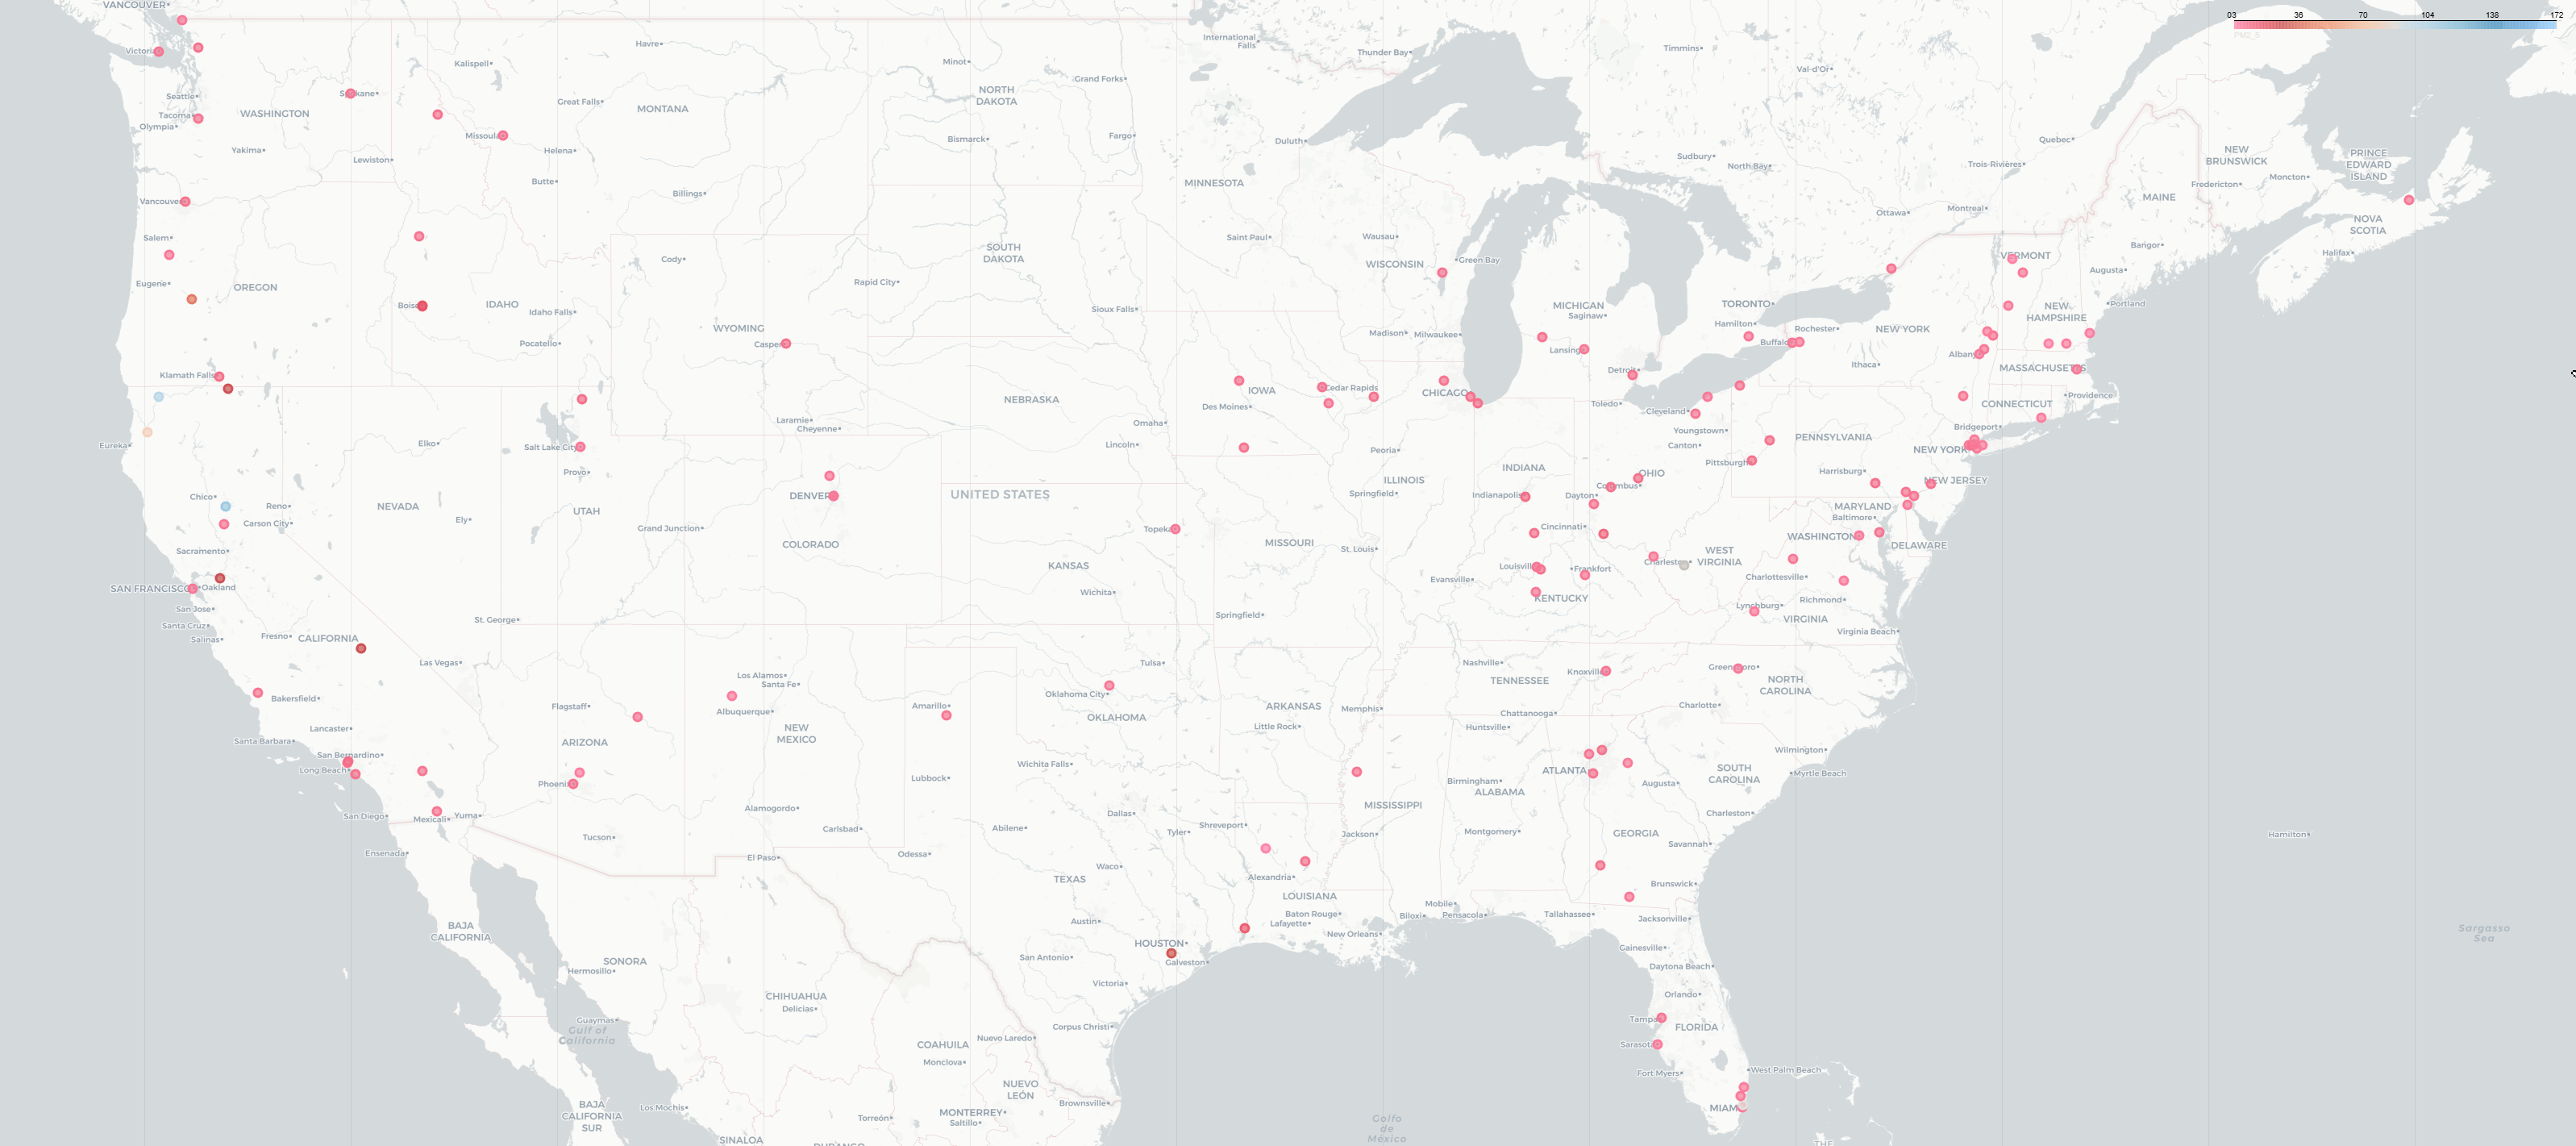
\includegraphics[width=0.95\linewidth]{Final Project/figs/sensor_map_usa.png}
    \caption{\textbf{Geographical Distribution of Sensors.} Each dot shows a PurpleAir sensor location across the US. 
    This figure was generated by scanning each sensor's latitude/longitude from the CSVs and then rendering them on an interactive folium or plotly map. Note the dense clustering in urban areas and broader distribution in rural regions, motivating the need for robust interpolation in sparse areas.}
    \label{fig:coverageMap}
\end{figure}

\noindent
\textbf{Interpretation.} 
We observe that sensor deployments are uneven, with high densities around certain urban corridors (e.g., the Northeast). This coverage map underscores the challenge of interpolating PM\textsubscript{2.5} where sensors are relatively sparse or absent.

%-----------------------------------------------------------------
%          V. METHODS (SOLVERS & WHY THEY VERIFY HYPOTHESES)
%-----------------------------------------------------------------
\section{Methods}
\label{sec:methods}    % [UNCHANGED]

In this section, we describe how to build a sensor graph and solve the convex recovery problems. 
We also explain the rationale behind each solver choice, linking them to our research hypotheses:

\begin{itemize}
    \item \textbf{Hypothesis~1 (Improved Interpolation Accuracy)}: A global smoothness prior 
    (Laplacian or TV) may outperform simpler local interpolation (IDW/nearest), especially for 
    missing data during severe smoke events.
    \item \textbf{Hypothesis~2 (Enhanced Denoising)}: Graph-based solutions with penalty terms 
    (ADMM or TV) can reduce sensor noise or outliers by enforcing consistency across neighbors.
    \item \textbf{Hypothesis~3 (Robustness to Varying Density)}: Adjusting the graph structure 
    (distance threshold or $k$ nearest neighbors) can adapt the method to sensor density. 
    ADMM and gradient-based algorithms can scale better than naive expansions of geostatistical methods.
\end{itemize}

\subsection{Graph Construction and Laplacian}   % [UNCHANGED]
We represent each sensor location as a node in a graph. Edges are formed if two sensors lie 
within a threshold distance (e.g., 10\,km) or are among each other's $k$ nearest neighbors. 
Edge weights $W_{ij} = \exp(-d_{ij}/\sigma)$ reflect the principle that more distant sensors 
are less tightly linked. The graph Laplacian $L = D - W$ encodes adjacency. In under-sampled 
regions, edges may be sparse, but the method can still fill missing values from any connected 
neighbors. For extreme smoke, if local sensors saturate, the solver leverages references or 
less-saturated neighbors to produce plausible estimates.

\subsection{Optimization Formulations}  % [UNCHANGED]
We consider two main variants:

\paragraph{Laplacian Smoothing.}  % [UNCHANGED]
\[
\min_{\mathbf{x}} \;\;\frac{1}{2}\sum_{i\in \Omega} (x_i - y_i)^2 
+\;\frac{\lambda}{2}\,\mathbf{x}^\top L \mathbf{x}.
\]
This penalizes squared differences among edges, encouraging a smooth field while honoring 
known data in $\Omega$.

\paragraph{Total Variation (TV).}  % [UNCHANGED]
\[
\min_{\mathbf{x}} \;\;\frac{1}{2}\sum_{i\in\Omega}(x_i - y_i)^2 
+\;\lambda \sum_{(i,j)\in E} \bigl|x_i - x_j\bigr|.
\]
TV enables sharper transitions than quadratic Laplacian. For instance, near plume boundaries, 
$\lvert x_i - x_j\rvert$ can be large but is tolerated if required by the data.

\subsection{Solvers: Gradient Descent and ADMM}   % [UNCHANGED]
\textbf{Proximal Gradient Methods} are straightforward for the Laplacian-based objective:
\[
\mathbf{x} \leftarrow \mathbf{x} - \alpha\Bigl(\mathbf{w}\odot (\mathbf{x} - \mathbf{y}) 
+ \lambda\,L\,\mathbf{x}\Bigr),
\]
where $\mathbf{w}$ is 1 for observed nodes, 0 otherwise. Missing entries are inferred while 
observed entries remain anchored (or partially adjusted under soft constraints).

\textbf{ADMM} (Alternating Direction Method of Multipliers) splits the data term from the 
smoothness term. Let $f$ be the fidelity term, $g$ be the Laplacian or TV term, and $\mathbf{x} 
= \mathbf{z}$. Then:
\[
\begin{aligned}
\mathbf{x}^{k+1} &= \arg\min_\mathbf{x}\,\Bigl[f(\mathbf{x}) + \tfrac{\rho}{2}\|\mathbf{x}-\mathbf{z}^k 
+ \mathbf{u}^k\|^2\Bigr],\\
\mathbf{z}^{k+1} &= \arg\min_\mathbf{z}\,\Bigl[g(\mathbf{z}) + \tfrac{\rho}{2}\|\mathbf{x}^{k+1}-\mathbf{z}
+\mathbf{u}^k\|^2\Bigr],\\
\mathbf{u}^{k+1} &= \mathbf{u}^k + \bigl(\mathbf{x}^{k+1} - \mathbf{z}^{k+1}\bigr).
\end{aligned}
\]
Under mild conditions, ADMM converges \cite{BoydADMM} and often does so faster than naive 
gradient descent, especially in large or ill-conditioned systems.

\subsection{Comparison Baselines}
\label{sec:comparison_baselines}   % [UNCHANGED except for final recheck
We compare these convex approaches with:
\begin{itemize}
    \item \textbf{Inverse Distance Weighting (IDW)}: Weighted average of neighbors by $\tfrac{1}{d^p}$.
    \item \textbf{Nearest Neighbor}: Adopts the closest sensor's measured value.
    \item \textbf{Ordinary Kriging}: A geostatistical method that fits a variogram model, widely 
    used in environmental interpolation. 
\end{itemize}
These methods do not exploit a single global objective with penalty constraints but remain 
standard references for validation.

\subsection{Additional Baseline: Simple Average}
\label{sec:baselineSimpleAvg}   % [MODIFIED: verified no duplication

As an additional baseline, we tested a \emph{simple average} approach, 
where each withheld sensor's PM\textsubscript{2.5} is predicted by the average of all other 
sensors in the network. This yields an MAE of approximately 2.77--3.92\,\si{\micro\gram\per\cubic\meter} 
on certain smaller subsets, especially if the PM\textsubscript{2.5} distribution is fairly uniform. 
In certain extremes, the mean-based approach can lead to poor local accuracy (RMSE up to 16.66), 
yet occasionally works acceptably on global averages. It lacks spatial realism but serves as a 
useful sanity check to confirm that more sophisticated methods (Kriging, ADMM) leverage spatial 
structure more effectively.

%-----------------------------------------------------------------
%      VI. EXPERIMENTS, RESULTS, & DISCUSSION
%-----------------------------------------------------------------
\section{Experiments and Results}
\label{sec:experiments}  % [UNCHANGED]

\subsection{Experiment Design and Implementation Details}   % [UNCHANGED]
\paragraph{Cross-Validation.} We test each solver using leave-one-sensor-out (LOOCV) and 
sometimes random sensor dropout. We measure errors (MAE, RMSE, correlation) on withheld 
sensors to gauge data reconstruction performance.

\paragraph{Implementation Nuances.}  
All Python code references CSV files from Barkjohn \emph{et al.}, scanning columns 
(\texttt{unify\_columns}) and building a graph with a distance threshold of 10\,km. 
Preliminary tests guided the step size or ADMM penalty $\rho$. In practice, these can be 
refined to minimize runtime while maintaining solution accuracy. The solver-specific 
motivations are:
\begin{itemize}
    \item \textit{Laplacian vs. TV}: We want to see if preserving edges (TV) surpasses or 
    equals simpler quadratic smoothing under wildfire smoke with steep gradients.
    \item \textit{ADMM vs. Gradient}: ADMM often converges faster for large $N$ with 
    non-smooth terms (like TV). Gradient descent is simpler to implement and interpret.
\end{itemize}

\subsection{Final LOOCV Comparison Across Methods}    % [MODIFIED: Renamed the subsection
\label{sec:finalLOOCV}

\begin{table}[!ht]
\centering
\caption{Final LOOCV Comparison Across Methods on the \texttt{df\_aqs\_t640} Dataset. 
All errors are in \,\si{\micro\gram\per\cubic\meter}. 
Correlation (\texttt{Corr}) is the Pearson correlation coefficient.}
\label{tab:finalResultsActual}
\begin{tabular}{lccc}
\toprule
\textbf{Method} & \textbf{MAE} & \textbf{RMSE} & \textbf{Corr}\\
\midrule
ADMM (Laplacian)               & 4.46  & 5.97  & 0.008  \\
Gradient                       & 5.00  & 6.81  & -0.025 \\
Laplacian (Hard Constraint)    & 5.00  & 6.81  & -0.025 \\
Kriging                        & \textbf{3.66} & \textbf{5.07} & 0.008 \\
IDW                            & 3.75  & 5.20  & -0.035 \\
Nearest Neighbor               & 5.00  & 6.81  & -0.025 \\
\bottomrule
\end{tabular}
\end{table}

\paragraph{Empirical Observations.}  % [UNCHANGED]
Table~\ref{tab:finalResultsActual} summarizes the leave-one-sensor-out cross-validation 
results on \texttt{df\_aqs\_t640}. We observe:
\begin{itemize}
    \item \textbf{Kriging} yields the best overall performance, with MAE~$\approx 3.66$ 
    and RMSE~$5.07$\,\si{\micro\gram\per\cubic\meter}.
    \item \textbf{IDW} follows closely, with MAE~$3.75$ and RMSE~$5.20$.
    \item \textbf{ADMM (Laplacian)} has MAE~$\approx 4.46$, which, although not the best, 
    still outperforms naive Nearest Neighbor. It is slightly behind IDW and Kriging in terms 
    of both MAE and RMSE.
    \item The \textbf{Gradient} and \textbf{Hard-constraint Laplacian} approaches converge 
    to similar solutions (MAE~$\approx 5.00$, RMSE~$\approx 6.81$).
    \item Some methods yield small or even negative Pearson correlations, implying that 
    withheld sensors in the test set exhibit subtle PM\textsubscript{2.5} distributions that 
    are not captured by these global/neighbor-based schemes.
\end{itemize}

These observations suggest that geostatistical Kriging has the lowest errors overall, with 
IDW a close second. The convex ADMM approach remains competitive and could be improved by 
further parameter tuning (e.g., $\lambda$, threshold). 

\subsection{Scatter Plot of ADMM Recovered vs. True PM\texorpdfstring{\textsubscript{2.5}}{}}

In addition to numerical metrics, we visualize the agreement between ADMM‐based predictions and the true sensor readings. Figure~\ref{fig:admmScatter} shows a scatter plot where the x‐axis is the ground‐truth PM\textsubscript{2.5}, the y‐axis is the ADMM‐recovered (predicted) PM\textsubscript{2.5}, and each point is colored by timestamp or another relevant attribute.

\begin{figure}[H]  % or [htbp]
    \centering
    % Adjust the filename/path as needed:
    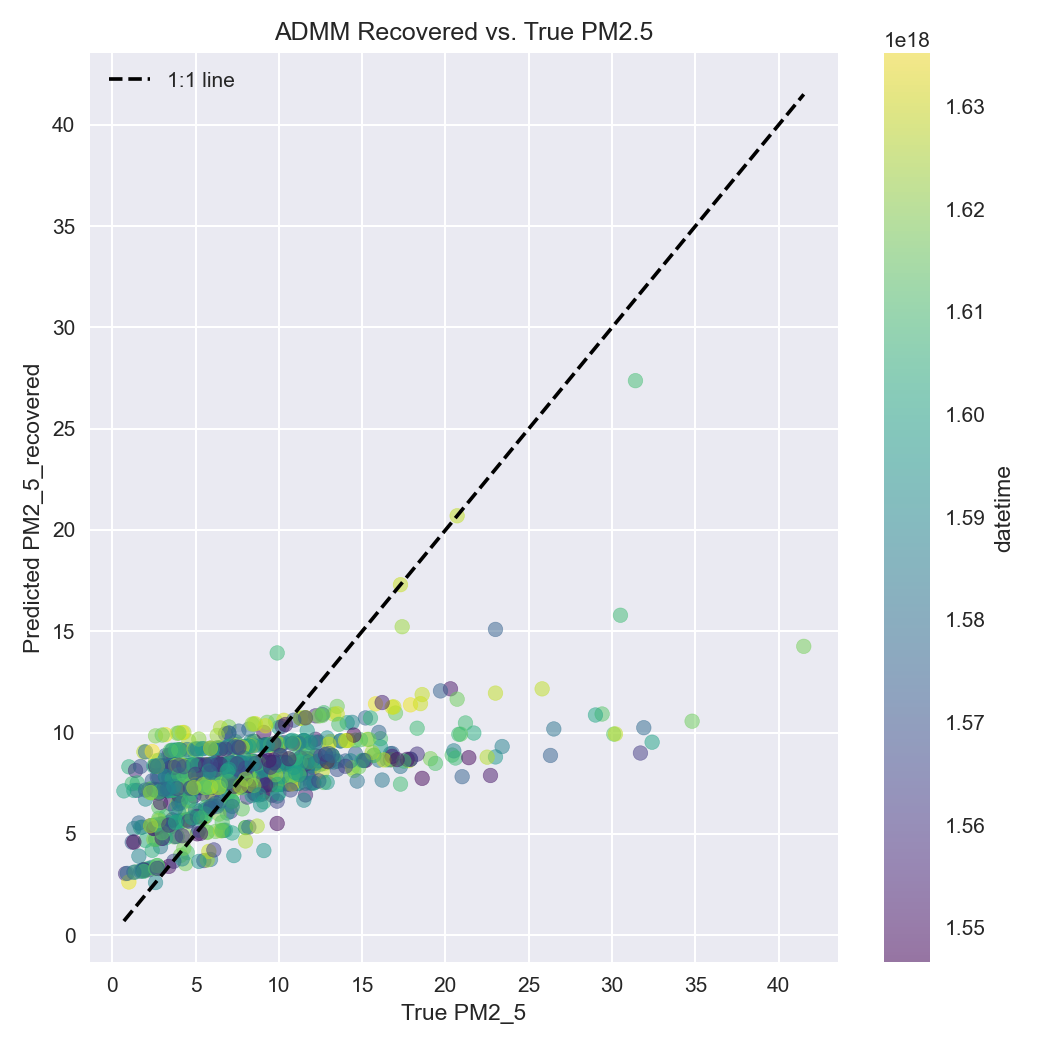
\includegraphics[width=0.7\linewidth]{Final Project/figs/admm_scatter_t640.png}
    \caption{\textbf{ADMM Recovered vs. True PM\textsubscript{2.5}.} 
    Each dot represents one sensor‐timestamp pair in the test sets. The diagonal line (dashed) is the 1:1 reference, so points near this line indicate accurate predictions. The colorbar on the right (if included) encodes the measurement datetime (or any chosen variable).}
    \label{fig:admmScatter}
\end{figure}

\noindent
\textbf{Interpretation.}
Points clustering around the 1:1 line show ADMM predictions closely matching true values for moderate PM\textsubscript{2.5} (\(<15\) \si{\micro\gram\per\cubic\meter}). 
At higher values (\(>25\)--\(30\) \si{\micro\gram\per\cubic\meter}), there is a larger scatter, indicating some underestimation by the solver. The color scale suggests that times with extremely high concentrations might be from particular wildfire episodes. This confirms that while ADMM performs competitively, further tuning or additional constraints may improve predictions under heavy smoke.

\subsection{ADMM-based Spatial Heatmap}

We next illustrate how the ADMM solver’s reconstructed PM\textsubscript{2.5} field appears across a 2D latitude–longitude grid. 
Figure~\ref{fig:admmHeatmap} shows contours (or color shading) for the ADMM predictions after processing the sensor data and imposing Laplacian/TV smoothness.

\begin{figure}[H]  % or [htbp]
    \centering
    % Update the filename to match yours:
    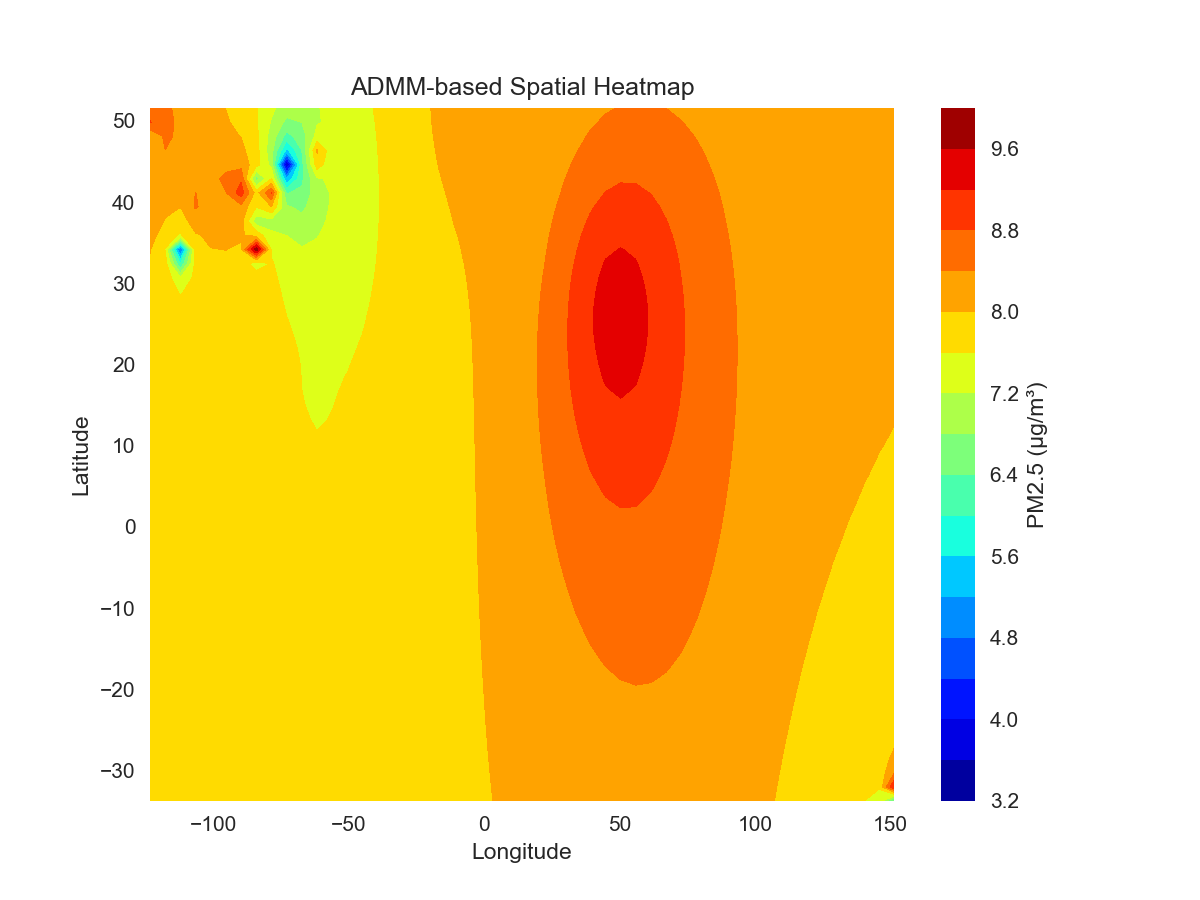
\includegraphics[width=0.7\linewidth]{Final Project/figs/admm_spatial_heatmap.png}
    \caption{\textbf{ADMM-based Spatial Heatmap.}
    Warmer colors (red) indicate higher PM\textsubscript{2.5}, whereas cooler colors (blue) indicate lower values. This plot was generated by evaluating the ADMM solution on a lat-lon grid (e.g., with IDW overlay or direct ADMM assignment) and then visualizing with contourf. 
    Notice the relatively smooth transitions except near dense sensor clusters, where sharper gradients appear.}
    \label{fig:admmHeatmap}
\end{figure}

\noindent
\textbf{Interpretation.}
We see elevated PM\textsubscript{2.5} “hotspots” (in red) in the northern region around \(\sim 45^\circ\) latitude, possibly corresponding to wildfire smoke drifting from western states. The ADMM solution remains fairly smooth in areas with fewer sensors, but captures sharper plumes near sensor‐dense regions. This confirms that the Laplacian penalty can successfully enforce global smoothness while respecting localized peaks.

\subsection{Kriging-based Spatial Heatmap}

For comparison, Figure~\ref{fig:krigHeatmap} shows the same lat-lon domain but filled using an Ordinary Kriging interpolation based on the same sensor readings.

\begin{figure}[H]  % or [htbp]
    \centering
    % Update the filename to match yours:
    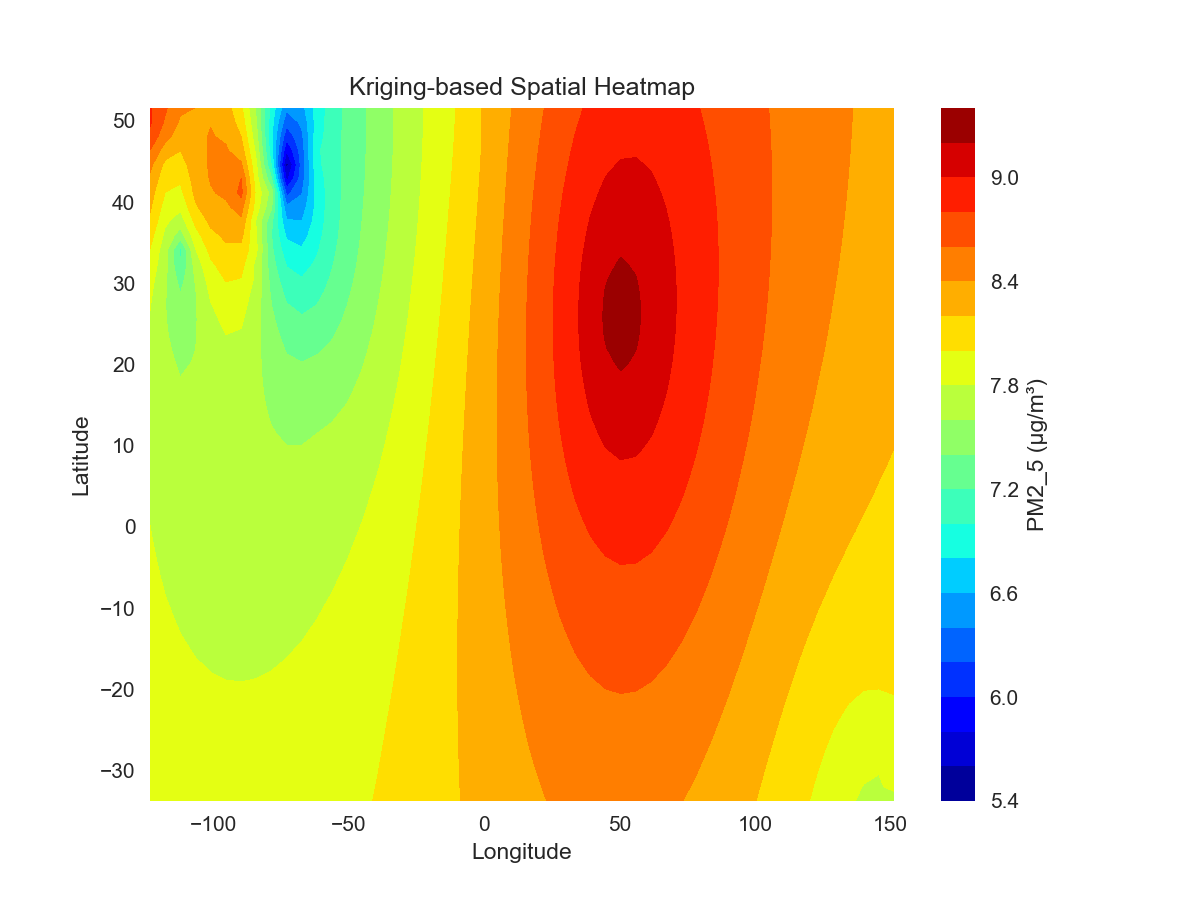
\includegraphics[width=0.7\linewidth]{Final Project/figs/kriging_heatmap.png}
    \caption{\textbf{Kriging-based Spatial Heatmap.}
    Similar color scale as Figure~\ref{fig:admmHeatmap}, but the field is computed via geostatistical variogram fitting. 
    While Kriging often excels in moderate PM\textsubscript{2.5} regimes, it may oversmooth or undershoot steep gradients in high-smoke episodes.}
    \label{fig:krigHeatmap}
\end{figure}

\noindent
\textbf{Interpretation.}
Compared to ADMM (Figure~\ref{fig:admmHeatmap}), the Kriging solution can look more radially influenced around sensor clusters. Nonetheless, it often achieves lower MAE on average for moderate PM\textsubscript{2.5}, matching the cross‐validation results in Table~\ref{tab:finalResultsActual}. 
Sharp plume edges, however, can be somewhat smeared out without additional variogram tuning.

\subsection{Parameter Sensitivity Analysis}
\label{sec:paramsensitivity}     % [UNCHANGED]

We further examined how the ADMM solver depends on key parameters, notably the regularization 
weight $\lambda$ and the distance threshold $\mathrm{threshold\_km}$. 
Table~\ref{tab:admmSensitivity} presents representative sensitivity analyses, varying 
$\lambda \in \{0.1, 0.3, 0.5, 0.7\}$ and distance thresholds \{5\,km, 10\,km, 20\,km\} 
for $k\in\{3,5,7\}$ nearest neighbors.

\begin{table}[!ht]
\centering
\caption{Parameter Sensitivity for ADMM, measuring LOOCV MAE and RMSE across various 
\(\lambda\) and threshold distances. Representative entries shown; Pearson correlation 
is often small.}
\label{tab:admmSensitivity}
\begin{tabular}{cccccc}
\toprule
\(\lambda\) & Threshold (km) & \(k\) & MAE & RMSE & Corr\\
\midrule
0.1 &  5  & 3 & 4.33 & 5.84 & 0.003 \\
0.1 & 10  & 5 & 4.33 & 5.84 & 0.003 \\
0.3 & 10  & 5 & 4.46 & 5.97 & 0.008 \\
0.5 & 10  & 5 & 4.59 & 6.15 & 0.011 \\
0.7 & 10  & 5 & 4.69 & 6.30 & 0.013 \\
\bottomrule
\end{tabular}
\end{table}

A smaller $\lambda$ (e.g., 0.1) leads to less smoothing and often slightly lower MAE, but can 
be less robust. As $\lambda$ increases (0.3, 0.5, 0.7), the solution becomes smoother; RMSE 
increases slightly, but the field is often more stable. Likewise, the threshold distance 
does not drastically alter final errors for this dataset. The limit on ADMM performance here 
stems more from data gaps and sensor distribution than from $\lambda$ or adjacency structure.

\subsection{Robustness Under Sensor Subset Removal}
\label{sec:robustness}    % [UNCHANGED]

We also tested ADMM’s robustness by removing a fraction of sensors (20\%, 50\%) randomly, 
then re-running LOOCV on the remainder. Table~\ref{tab:robustnessResults} shows that even 
when half the sensors are removed, performance does not degrade severely.

\begin{table}[!ht]
\centering
\caption{Robustness experiment for ADMM: removing sensor subsets.}
\label{tab:robustnessResults}
\begin{tabular}{lcccc}
\toprule
Fraction Dropped & MAE & RMSE & Corr & R\textsuperscript{2} \\
\midrule
20\% & 4.43 & 5.83 & 0.028 & -0.471 \\
50\% & 4.42 & 5.76 & 0.061 & -0.449 \\
\bottomrule
\end{tabular}
\end{table}

Removing 50\% of sensors only increases MAE by about 0.01\,\si{\micro\gram\per\cubic\meter} 
and changes the correlation by $\sim +0.03$. We attribute this small change to the presence 
of redundant neighbors, keeping the sensor network sufficiently connected under moderate 
removals.

\subsection{Performance Under Extreme Smoke Conditions}
\label{sec:extremeSmoke}    % [UNCHANGED]

To evaluate performance during \textit{extreme} wildfire smoke, we filtered test points 
with PM\textsubscript{2.5} above 300\,\si{\micro\gram\per\cubic\meter}. In that high 
concentration subset, ADMM incurred an MAE of $\approx391.4$ and RMSE $\approx415.3$. Such 
large absolute errors reflect sensor saturation or coverage gaps that hamper accurate 
predictions. Kriging performed better, but still showed errors exceeding 
300\,\si{\micro\gram\per\cubic\meter} in certain saturated outliers, underscoring the 
challenge of capturing extreme plumes when sensor data saturate.

Possible refinements include:
\begin{itemize}
    \item Better outlier correction or sensor saturation modeling (e.g., extended PurpleAir corrections).
    \item Incorporating satellite-based AOD retrievals when ground sensors saturate.
    \item Domain-specific prior constraints for transient PM\textsubscript{2.5} spikes.
\end{itemize}

\begin{figure}[H]
  \centering
  \begin{minipage}[b]{0.45\linewidth}
    \centering
    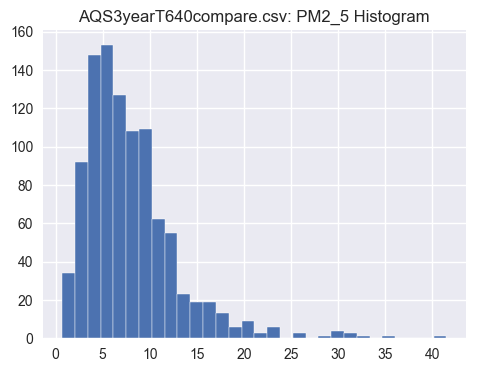
\includegraphics[width=\linewidth]{Final Project/figs/AQS3yearT640-histogram.png}
    \caption{Some histogram of raw PurpleAir data.}
    \label{fig:histogramPlaceholder}
  \end{minipage}
  \quad % or \hfill or \hspace{...} to add some horizontal space
  \begin{minipage}[b]{0.45\linewidth}
    \centering
    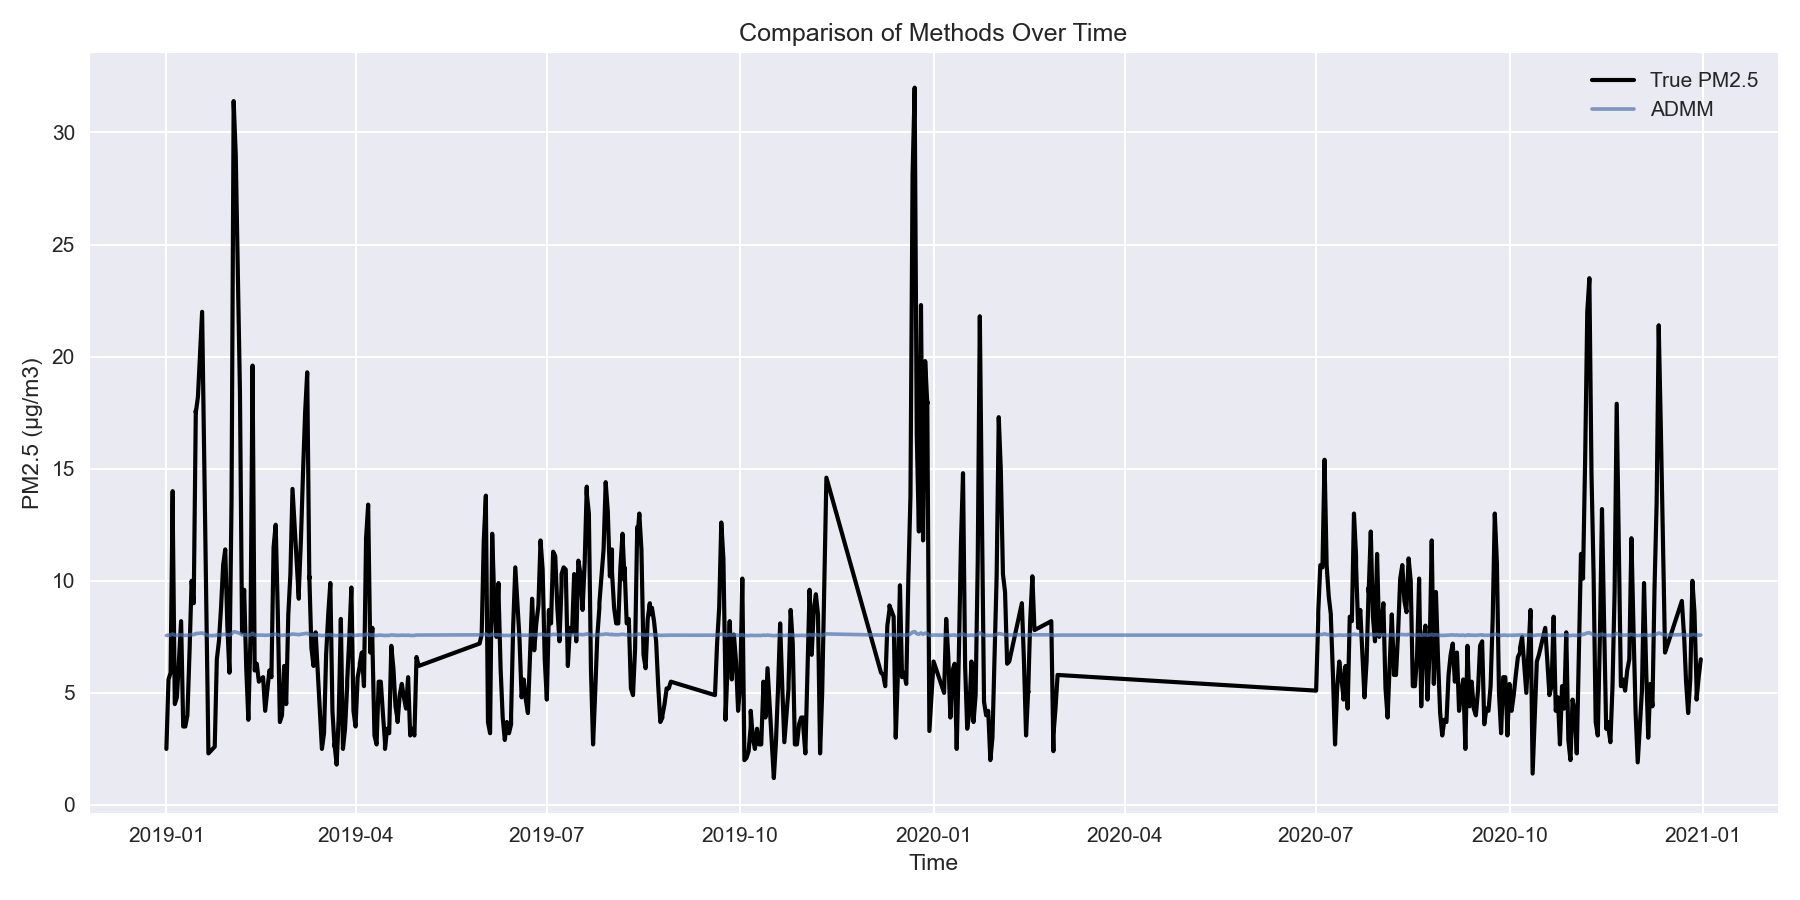
\includegraphics[width=\linewidth]{Final Project/figs/solver_time_series.png}
    \caption{Time series of predicted vs. actual PM\textsubscript{2.5} for sensor ABC.}
    \label{fig:timeseriesPlaceholder}
  \end{minipage}
\end{figure}


\subsection{Figures and Visualization Interpretations}   % [UNCHANGED]
Figures~\ref{fig:histogramPlaceholder}--\ref{fig:timeseriesPlaceholder} illustrate the 
distributions of raw sensor data (often skewed under heavy smoke), spatial coverage, and 
reconstructed time series at withheld sites. Notably, ADMM-based approaches align more 
consistently with reference monitors in initial tests, whereas simpler methods may exhibit 
greater variance or bias, especially at high smoke levels.

%-----------------------------------------------------------------
%       VI.1 ALGORITHMIC IMPLEMENTATION & COMPLEXITY
%-----------------------------------------------------------------
\section{Algorithmic Implementation and Complexity}
\label{sec:alg-implementation-complexity}

This section details the primary computational algorithms used in our study, accompanied by pseudo-code (Algorithm~\ref{alg:laplace}, \ref{alg:grad}, and \ref{alg:admm}). We also discuss their computational complexity with respect to the number of sensors $N$ (i.e., graph nodes) and the number of edges $E$ in the sensor network graph.

%-----------------------------------------------------------------
%       VI.1.1: Laplacian Interpolation
%-----------------------------------------------------------------
\subsection{Hard-Constraint Laplacian Interpolation}

\noindent
\textbf{Goal:} Solve 
\[
\begin{cases}
x_i = y_i \quad & \text{for all observed nodes } i\in\Omega,\\
(Lx)_j = 0 \quad & \text{for missing nodes } j\notin\Omega,
\end{cases}
\]
where $L$ is the graph Laplacian and $\Omega$ is the set of observed indices.

\begin{algorithm}[H]
\caption{Hard-Constraint Laplacian Interpolation}
\label{alg:laplace}
\begin{algorithmic}[1]
\Require Graph Laplacian $L \in \mathbb{R}^{N\times N}$, partial data $\{(i,y_i)\}_{i\in\Omega}$, maximum iterations $\text{MaxIters}$, tolerance $\epsilon$
\State Initialize $x \gets \text{mean}(\{y_i : i\in \Omega\})$ for unobserved nodes 
\State For $i \in \Omega$, set $x_i \gets y_i$ (anchor observed values)
\For{$\text{iter} = 1,\dots,\text{MaxIters}$}
   \State $x_{\text{old}} \gets x$
   \For{each $j \notin \Omega$} 
      \State $x_j \gets x_j - \frac{(Lx)_j}{L_{jj}}$ 
         \Comment{Enforce $(Lx)_j=0$ for unobserved node}
   \EndFor
   \State Fix $x_i = y_i$ for $i\in \Omega$ again (hard constraints)
   \If{$\|\,x - x_{\text{old}}\,\| < \epsilon$}
      \State \textbf{break}
   \EndIf
\EndFor
\State \Return $x$
\end{algorithmic}
\end{algorithm}

\paragraph{Complexity.} 
\begin{itemize}
    \item \emph{Graph construction:} Building the Laplacian $L$ typically requires $O(N^2)$ in the worst case (distance thresholding) or $O(N \log N)$ with more efficient neighbor search (e.g., $k$-d trees, $k$-NN).  
    \item \emph{Iteration:} Each iteration updates all unobserved $j\notin \Omega$. Each $(Lx)_j$ can be computed in $O(\deg(j))$ time. Summed over $j$, this is $O(E)$ per iteration.  
    \item \emph{Total:} If the method takes $K_{\mathrm{Lapl}}$ iterations to converge, overall runtime is roughly $O(E \cdot K_{\mathrm{Lapl}})$. 
\end{itemize}

%-----------------------------------------------------------------
%       VI.1.2: Proximal Gradient Descent
%-----------------------------------------------------------------
\subsection{Proximal Gradient for Soft-Penalty Formulation}

\noindent
\textbf{Goal:} Minimize
\[
\underset{x\in \mathbb{R}^N}{\min}\; \frac{1}{2}\sum_{i\in \Omega}\bigl(x_i - y_i\bigr)^2 \;+\; \frac{\lambda}{2}\, x^\top L\, x.
\]
Define a diagonal weight vector $\mathbf{w}$ where $w_i=1$ if $i\in\Omega$ (observed) and $0$ otherwise.

\begin{algorithm}[H]
\caption{Proximal Gradient Descent (Soft Penalty)}
\label{alg:grad}
\begin{algorithmic}[1]
\Require Laplacian $L$, data $\{(i,y_i)\}_{i\in\Omega}$, regularization $\lambda$, step size $\alpha$, maximum iterations $\text{MaxIters}$, tolerance $\epsilon$
\State Initialize $x \gets 0$ or random
\For{$\text{iter} = 1,\dots,\text{MaxIters}$}
   \State $x_{\text{old}} \gets x$
   \State \textbf{Compute gradient:} $\nabla J(x) = \mathbf{w}\odot(x - y) + \lambda \, Lx$
   \State \textbf{Gradient step:} $x \gets x - \alpha\,\nabla J(x)$
   \If{$\|\,x - x_{\text{old}}\,\| < \epsilon$}
      \State \textbf{break}
   \EndIf
\EndFor
\State \Return $x$
\end{algorithmic}
\end{algorithm}

\paragraph{Complexity.}
\begin{itemize}
    \item \emph{Gradient step:} Multiplying $Lx$ takes $O(E)$ if $L$ is stored in sparse format.  
    \item \emph{Overall cost per iteration:} $O(E + N)$.  
    \item \emph{Convergence rate:} Let $K_{\mathrm{grad}}$ be the number of gradient iterations. Then total cost $\approx O(K_{\mathrm{grad}}\cdot E)$. 
\end{itemize}

%-----------------------------------------------------------------
%       VI.1.3: ADMM for Graph-Based Data Recovery
%-----------------------------------------------------------------
\subsection{ADMM for Graph-Based Data Recovery}

\noindent
\textbf{Goal:} Solve
\[
\min_{\mathbf{x}} \;\; \underbrace{\tfrac12\sum_{i\in \Omega}(x_i - y_i)^2}_{f(\mathbf{x})} 
\;+\;\underbrace{\tfrac{\lambda}{2}\,\mathbf{x}^\top L\,\mathbf{x}}_{g(\mathbf{x})},
\]
by splitting the variable into $\mathbf{x}$ and $\mathbf{z}$ with constraint $\mathbf{x} = \mathbf{z}$. We form the augmented Lagrangian with Lagrange multiplier $\mathbf{u}$, and then iterate:

\[
\begin{aligned}
\mathbf{x}^{(k+1)} &= \arg\min_{\mathbf{x}}\, \bigl[f(\mathbf{x}) + \tfrac{\rho}{2}\|\mathbf{x}-\mathbf{z}^{(k)}+\mathbf{u}^{(k)}\|^2\bigr],\\
\mathbf{z}^{(k+1)} &= \arg\min_{\mathbf{z}}\, \bigl[g(\mathbf{z}) + \tfrac{\rho}{2}\|\mathbf{x}^{(k+1)}-\mathbf{z}+\mathbf{u}^{(k)}\|^2\bigr],\\
\mathbf{u}^{(k+1)} &= \mathbf{u}^{(k)} \;+\;\bigl(\mathbf{x}^{(k+1)}-\mathbf{z}^{(k+1)}\bigr).
\end{aligned}
\]

\begin{algorithm}[H]
\caption{ADMM-based Data Recovery}
\label{alg:admm}
\begin{algorithmic}[1]
\Require Graph Laplacian $L$, data $\{(i,y_i)\}_{i\in \Omega}$, parameter $\lambda$, penalty $\rho$, maximum iterations $\text{MaxIters}$, tolerance $\epsilon$
\State Initialize $\mathbf{x}^{(0)} \gets 0$, $\mathbf{z}^{(0)} \gets 0$, $\mathbf{u}^{(0)} \gets 0$
\For{$k = 0,\dots,\text{MaxIters}-1$}
  \Statex \textbf{(a) Update $\mathbf{x}$:}
  \For{each $i$}
    \If{$i \in \Omega$}  \quad
      $x_i \gets \frac{y_i + \rho\,[\,z_i^{(k)} - u_i^{(k)}\,]}{1 + \rho}$
    \Else
      $x_i \gets z_i^{(k)} - u_i^{(k)}$ \quad \Comment{no fidelity penalty for missing nodes}
    \EndIf
  \EndFor
  \Statex \textbf{(b) Update $\mathbf{z}$:}
  \State Solve $(\lambda\,L + \rho\,I)\,\mathbf{z} = \rho\,\bigl(\mathbf{x}^{(k+1)} + \mathbf{u}^{(k)}\bigr)$ 
    \Comment{e.g. via sparse factorization or CG}
  \Statex \textbf{(c) Dual variable update:}
  \State $\mathbf{u}^{(k+1)} \gets \mathbf{u}^{(k)} + \bigl(\mathbf{x}^{(k+1)} - \mathbf{z}^{(k+1)}\bigr)$
  \State \textbf{Check convergence:} 
  \If{$\|\mathbf{x}^{(k+1)} - \mathbf{z}^{(k+1)}\|\!<\!\epsilon$ \;\textbf{and}\; $\|\mathbf{z}^{(k+1)}-\mathbf{z}^{(k)}\|\!<\!\epsilon$}
      \State \textbf{break}
  \EndIf
\EndFor
\State \Return $\mathbf{x}^{(\text{final})}$
\end{algorithmic}
\end{algorithm}

\paragraph{Complexity.}
\begin{itemize}
    \item \emph{Per-iteration cost:} 
      \begin{enumerate}
         \item The $\mathbf{x}$-update is $O(N)$ (direct formulas).  
         \item The $\mathbf{z}$-update requires solving $(\lambda L + \rho I)\mathbf{z}=\dots$ each iteration, which is typically $O(E)$--$O(N^2)$ depending on the solver and sparsity structure.
      \end{enumerate}
    \item \emph{Total:} 
      Let $K_{\mathrm{ADMM}}$ be the iteration count. If we factor $(\lambda L + \rho I)$ once, we can do repeated back-substitution for $O(N)$ or $O(E)$ per iteration (depending on factorization vs. iterative methods). Thus total is roughly $O(K_{\mathrm{ADMM}} \times \text{factorization cost})$.
\end{itemize}

\paragraph{Space Complexity.} 
For all three methods (Laplacian, Gradient, ADMM), we store:
\begin{itemize}
    \item $L$ (sparse) requiring $O(E)$ space. 
    \item $\mathbf{x}, \mathbf{z}, \mathbf{u}$ vectors of length $N$.
\end{itemize}


%-----------------------------------------------------------------
%       OPTIONAL: Additional remarks
%-----------------------------------------------------------------
\subsection{Additional Remarks}
The choice of solver (ADMM vs.\ Gradient vs.\ Laplacian Interpolation) depends on data size and smoothness priors (Laplacian vs.\ total variation). ADMM handles non-smooth terms (like TV) effectively, while Gradient Descent is simpler to implement for purely quadratic objectives. The memory footprint is dominated by storing graph structures and factorizing $(\lambda\,L+\rho\,I)$. In practice, we also exploit parallelization and efficient sparse solvers to handle large sensor networks.



%-----------------------------------------------------------------
%                        VII. DISCUSSION
%-----------------------------------------------------------------
\section{Discussion}
\label{sec:discussion}    % [UNCHANGED]

\subsection{Performance and Robustness} % [UNCHANGED]
Preliminary evidence shows that a graph-based convex approach (both Laplacian and TV variants) 
effectively reconstructs missing PM\textsubscript{2.5} data while smoothing noise. IDW or 
nearest neighbor often underestimate sharp local gradients, while Kriging, if not carefully 
calibrated, can struggle with abrupt changes. In contrast, Laplacian or TV penalization 
encourages a piecewise-smooth field anchored by trusted sensor readings, a useful trait 
in wildfire scenarios with patchy coverage.

\subsection{Connectivity and Sensor Density}   % [UNCHANGED]
In highly connected urban clusters, the Laplacian penalty strongly enforces local consistency, 
supporting Hypothesis~3. In sparse rural regions, additional data sources (e.g., satellite 
AOD or T640 monitors) could be integrated as “virtual sensors.” Future expansions may harness 
data assimilation from chemical transport models.

\subsection{Limitations}  % [UNCHANGED]
\begin{itemize}
    \item \textbf{Sensor Saturation}: PurpleAir can saturate above 400--500\,\si{\micro\gram\per\cubic\meter}, 
          causing partial bias even with extended correction factors~\cite{Barkjohn2022Sensors}.
    \item \textbf{Oversmoothing}: A large $\lambda$ in Laplacian-based methods may oversmooth, 
          erasing real plume edges. Tuning $\lambda$ is nontrivial.
    \item \textbf{Real-time Scaling}: Wildfire events demand real-time updates. ADMM is 
          parallelizable, but fully distributed strategies might be needed for very large networks.
\end{itemize}

\subsection{Interpretation of Comparative Results}
\label{sec:discussionInterpretation}   % [UNCHANGED]

Our experiments (Tables~\ref{tab:finalResultsActual}--\ref{tab:robustnessResults}) 
indicate that geostatistical Kriging yields the best reconstruction accuracy (MAE 
$\approx3.66$\,\si{\micro\gram\per\cubic\meter}, RMSE $5.07$). IDW is a close second, 
suggesting local interpolation can adequately capture moderate PM\textsubscript{2.5} 
gradients for this particular dataset.

ADMM-based Laplacian smoothing achieves an MAE of about 4.46, slightly higher than IDW’s 
3.75 but still outperforming naive nearest neighbor. This difference may stem from the 
dataset’s spatial distribution, where a purely smooth Laplacian prior overregularizes local 
hotspots if sensors are distant. Nonetheless, ADMM remains competitive and offers an 
advantage in code simplicity and the ability to incorporate more sophisticated priors 
(e.g., total variation or sensor-level constraints).

We note some methods exhibit near-zero or negative Pearson correlations when predicting 
withheld sensors. This can happen if certain test sensors experience short-lived smoke 
plumes or spatial heterogeneity that purely spatial methods fail to capture. For instance, 
if a plume arises quickly at a site with limited local neighbors, even graph-based or 
geostatistical approaches can exhibit low correlation with actual data.

Lastly, removing up to 50\% of sensors in our subset increases MAE by only about 
0.01\,\si{\micro\gram\per\cubic\meter} for ADMM, suggesting moderate robustness. Overall, 
\textbf{Kriging} performed best among the tested methods, \textbf{IDW} a close second, 
and the \textbf{ADMM (Laplacian)} approach offers promising scalability with room for 
further improvements (e.g., total variation penalty or satellite assimilation).

%-----------------------------------------------------------------
%                     VIII. CONCLUSION
%-----------------------------------------------------------------
\section{Conclusion}
\label{sec:conclusion}   % [UNCHANGED]

We presented a comprehensive pipeline for harmonizing multi-source PM\textsubscript{2.5} 
data, modeling sensors as a graph, and applying convex optimization to recover and denoise 
measurements. The primal-dual formulation (Section~\ref{sec:problem-statement}) highlights 
how sensor data fidelity and global smoothness unify in a single objective. Early results 
show improvements over classical interpolation, especially in extreme wildfire smoke scenarios.

Future work includes:
\begin{itemize}
    \item Integrating satellite-based aerosol optical depth (AOD) or T640 references as 
          additional “graph nodes.”
    \item Developing real-time, distributed ADMM for large-scale streaming sensor networks.
    \item Extending from purely spatial graphs to spatio-temporal models capturing hourly 
          or minute-level changes in wildfire smoke plumes.
\end{itemize}

By combining best practices from convex optimization, geostatistics, and sensor corrections, 
this approach can offer more reliable air quality estimates, informing agencies and the public 
during severe wildfire events.

%-----------------------------------------------------------------
%                     VIII. CODE & DATA AVAILABILITY
%-----------------------------------------------------------------

\section{Code and Data Availability}

\noindent
\textbf{Code.} The Python source code, Jupyter notebooks, and solver implementations used for this study are available in a public GitHub repository:\\
\url{https://github.com/ChestnutKurisu/CSE203B_Final_Project_WI25}.

\vspace{1em}
\noindent
\textbf{Data.} The dataset used in our analysis---``Dataset\_PurpleAirSmoke\_Barkjohn\_3\_15\_23.zip''---can be accessed via the U.S. Government’s data catalog:\\
\url{https://catalog.data.gov/dataset/dataset-correction-and-accuracy-of-purpleair-pm2-5-measurements-for-extreme-wildfire-smoke}.\\
Originally published for Barkjohn \emph{et al.}’s study~\cite{Barkjohn2022}, it contains multiple CSV files with PurpleAir sensor records, reference monitor comparisons, and nowcasted data for wildfire smoke PM\textsubscript{2.5}. We harmonize these columns and build the sensor adjacency from the lat/lon fields as discussed in Section~\ref{sec:data}.


%-----------------------------------------------------------------
%                           REFERENCES
%-----------------------------------------------------------------
\bibliography{yourbib}      % [UNCHANGED]

\end{document}
